% !TEX TS-program = XeLaTeX
% use the following command:
% all document files must be coded in UTF-8
\documentclass[portuguese]{textolivre}
% build HTML with: make4ht -e build.lua -c textolivre.cfg -x -u article "fn-in,svg,pic-align"

\journalname{Texto Livre}
\thevolume{16}
%\thenumber{1} % old template
\theyear{2023}
\receiveddate{\DTMdisplaydate{2023}{7}{17}{-1}} % YYYY MM DD
\accepteddate{\DTMdisplaydate{2023}{9}{20}{-1}}
\publisheddate{\today}
\corrauthor{Joao Carlos Sousa}
\articledoi{10.1590/1983-3652.2023.46902}
%\articleid{NNNN} % if the article ID is not the last 5 numbers of its DOI, provide it using \articleid{} commmand 
% list of available sesscions in the journal: articles, dossier, reports, essays, reviews, interviews, editorial
\articlesessionname{reviews}
\runningauthor{Sousa} 
%\editorname{Leonardo Araújo} % old template
\sectioneditorname{Daniervelin Pereira}
\layouteditorname{Leonardo Araújo}

\title{Resenha de Designing for democracy: how to build community in digital environments}
\othertitle{Review of Designing for democracy: how to build community in digital environments}
% if there is a third language title, add here:
%\othertitle{Artikelvorlage zur Einreichung beim Texto Livre Journal}

\author[1]{Joao Carlos Sousa~\orcid{0000-0002-7374-0152}\thanks{Email: \href{mailto:joao.carlos.sousa@iscte-iul.pt}{joao.carlos.sousa@iscte-iul.pt}}}
\affil[1]{Instituto Universitário de Lisboa, Centro de Investigação e Estudos em Sociologia, Lisboa, Portugal.}

\addbibresource{article.bib}
% use biber instead of bibtex
% $ biber article

% used to create dummy text for the template file
\definecolor{dark-gray}{gray}{0.35} % color used to display dummy texts
\usepackage{lipsum}
\SetLipsumParListSurrounders{\colorlet{oldcolor}{.}\color{dark-gray}}{\color{oldcolor}}

% used here only to provide the XeLaTeX and BibTeX logos
\usepackage{hologo}

% if you use multirows in a table, include the multirow package
\usepackage{multirow}

% provides sidewaysfigure environment
\usepackage{rotating}

% CUSTOM EPIGRAPH - BEGIN 
%%% https://tex.stackexchange.com/questions/193178/specific-epigraph-style
\usepackage{epigraph}
\renewcommand\textflush{flushright}
\makeatletter
\newlength\epitextskip
\pretocmd{\@epitext}{\em}{}{}
\apptocmd{\@epitext}{\em}{}{}
\patchcmd{\epigraph}{\@epitext{#1}\\}{\@epitext{#1}\\[\epitextskip]}{}{}
\makeatother
\setlength\epigraphrule{0pt}
\setlength\epitextskip{0.5ex}
\setlength\epigraphwidth{.7\textwidth}
% CUSTOM EPIGRAPH - END

% LANGUAGE - BEGIN
% ARABIC
% for languages that use special fonts, you must provide the typeface that will be used
% \setotherlanguage{arabic}
% \newfontfamily\arabicfont[Script=Arabic]{Amiri}
% \newfontfamily\arabicfontsf[Script=Arabic]{Amiri}
% \newfontfamily\arabicfonttt[Script=Arabic]{Amiri}
%
% in the article, to add arabic text use: \textlang{arabic}{ ... }
%
% RUSSIAN
% for russian text we also need to define fonts with support for Cyrillic script
% \usepackage{fontspec}
% \setotherlanguage{russian}
% \newfontfamily\cyrillicfont{Times New Roman}
% \newfontfamily\cyrillicfontsf{Times New Roman}[Script=Cyrillic]
% \newfontfamily\cyrillicfonttt{Times New Roman}[Script=Cyrillic]
%
% in the text use \begin{russian} ... \end{russian}
% LANGUAGE - END

% EMOJIS - BEGIN
% to use emoticons in your manuscript
% https://stackoverflow.com/questions/190145/how-to-insert-emoticons-in-latex/57076064
% using font Symbola, which has full support
% the font may be downloaded at:
% https://dn-works.com/ufas/
% add to preamble:
% \newfontfamily\Symbola{Symbola}
% in the text use:
% {\Symbola }
% EMOJIS - END

% LABEL REFERENCE TO DESCRIPTIVE LIST - BEGIN
% reference itens in a descriptive list using their labels instead of numbers
% insert the code below in the preambule:
%\makeatletter
%\let\orgdescriptionlabel\descriptionlabel
%\renewcommand*{\descriptionlabel}[1]{%
%  \let\orglabel\label
%  \let\label\@gobble
%  \phantomsection
%  \edef\@currentlabel{#1\unskip}%
%  \let\label\orglabel
%  \orgdescriptionlabel{#1}%
%}
%\makeatother
%
% in your document, use as illustraded here:
%\begin{description}
%  \item[first\label{itm1}] this is only an example;
%  % ...  add more items
%\end{description}
% LABEL REFERENCE TO DESCRIPTIVE LIST - END


% add line numbers for submission
%\usepackage{lineno}
%\linenumbers

\begin{document}
\maketitle

\begin{figure}[htbp]
 \centering
 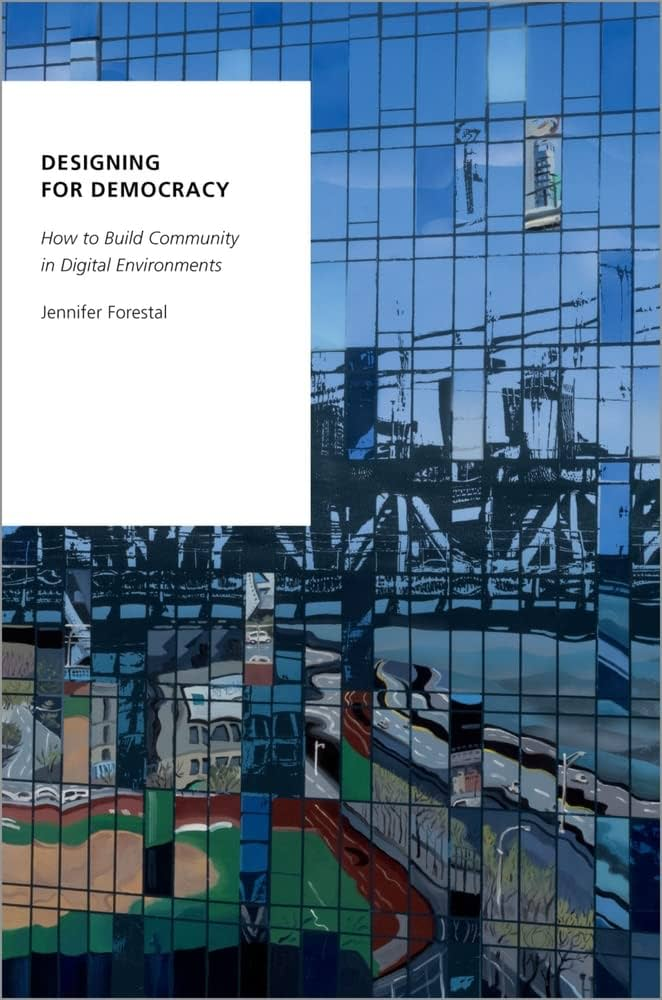
\includegraphics[width=0.5\textwidth]{Fig1.jpg}
 \caption*{\fullcite{forestal_designing_2021}}
 %\caption{\fullcite{nascimento_formacao_2019}.}
 \label{fig01}
% \source{fonte.}
\end{figure}

O trabalho de Jennifer Forestal (Loyola University Chicago) situa-se entre a arquitetura e a mudança cultural em contexto digital. Os seus interesses de investigação versam sobre os efeitos culturais e políticos dos espaços digitais. O modelo participativo de \textcite{dewey_democracy_2015} serve de eixo norteador do seu pensamento. \textit{Designing for Democracy} representa um disruptivo contributo para a abordagem da cultura e da política digital. A obra organiza-se em seis capítulos, redigidos em tom ensaístico seguindo um método compreensivo.

No primeiro capítulo, a autora debruça-se sobre o impacto da arquitetura dos espaços digitais na participação cívica e política. A obra tem como indagação inicial: como as plataformas digitais facilitam práticas democráticas?

O aumento da preponderância dos ambientes construídos promove sentimentos de perda de poder por parte dos cidadãos, criando condições para: racismo; desinformação; discursos de ódio e radicalização ideológica. As escolhas do \textit{design} das plataformas têm o poder de transformar a cultura e as atitudes dos utilizadores levando-os a agir de modo diferente.

Para que a participação cívica e política seja possível, os espaços digitais construídos devem garantir três condições: a existência prévia de uma comunidade; a sua sustentabilidade ao longo do tempo e existência de mecanismos autocorretores. Um espaço para ser considerado um local propiciador de uma cultura democrática deverá garantir três dimensões: delimitados; duráveis e flexível. A delimitação dos espaços, com fronteiras perfeitamente identificáveis, potencia a partilha e o reconhecimento com quem se partilha. A durabilidade dos espaços possibilita a sustentação temporal das comunidades que se formam nas plataformas digitais como o Twitter. O processo democrático implica confiança e informalidade, pelo que a flexibilidade dos espaços construídos é fundamental para promover aquilo a que a autora designa por \textit{hábito experimental}. Esse conceito envolve vontade de rever as próprias decisões, através da mudança intelectual, da curiosidade e da desenvoltura. Por conseguinte, a concepção de democracia da autora é enunciada nos seguintes termos: “[...] um modo de vida – um conjunto de práticas, atitudes e relações que (devemos) levar para todas as esferas de atividade que partilhamos com os outros” \cite[p. 24, tradução nossa]{forestal_designing_2021}. Desse modo, potencia-se a participação de todos os cidadãos, na vida comunitária e, com isso, nas mais diversas esferas da vida quotidiana.

Os espaços digitais democráticos, para se constituírem enquanto tal, deverão comportar os seguintes eixos estruturantes: fronteiras que dizem respeito às opções do próprio \textit{design} da plataforma e que podem facilitar ou constranger a emergência de amizades políticas entre os utilizadores; uma comunidade, mesmo que no espaço digital necessite de uma certa durabilidade – essa sustentabilidade ao longo do tempo é condição fundamental para uma qualquer comunidade política frutificar; finalmente, os espaços digitais construídos devem também garantir alguma flexibilidade, possibilitando a maleabilidade e diversidade de práticas \textit{on-line} e estimulando o hábito experimental. O capítulo encerra com a autora a advogar uma necessária discussão política sobre a propriedade das plataformas digitais e os efeitos políticos dos algoritmos.

No segundo capítulo, alega-se a relevância de fronteiras que possibilitam o reconhecimento de interesses e de concidadãos, além de potenciar a responsabilização coletiva, permitindo fomentar amizades políticas e comunidades democráticas. Um exemplo da relevância das fronteiras é o Facebook, que, ao eliminá-las, promove maior transparência; privatização das relações um-a-um; exacerbação da individualização; e cultura mais aberta. A consequência é a intensificação de uma cultura de individualismo em rede, em que uma pessoa é o centro da sua própria rede de comunicação, separada das demais, tendo como implicação a desconfiança política.

O mote do terceiro capítulo é dado pela autora através da definição do problema analítico, que consiste na sustentação das comunidades políticas \textit{on-line} ao longo do tempo. Não obstante as plataformas digitais serem espaços construídos que potenciam a mobilização, a verdade é que esses mesmos espaços já não oferecem condições que propiciem a durabilidade e sustentação de uma comunidade política ao longo do tempo. Nesse âmbito, a autora vai mais além e assume algumas sugestões de forma a mitigar essa tendência, nomeadamente proporcionar o reconhecimento de interesses em comum; o reconhecimento dos seus concidadãos; e, ainda, o incentivo a práticas cívicas que se baseiem no experimentalismo.

A esse respeito, o Twitter constitui-se como uma relevante plataforma digital nas sociedades contemporâneas por facilitar a identificação tanto de interesses como de concidadãos. Contudo, notabiliza-se como um espaço que não fomenta o estabelecimento de relações e laços entre os utilizadores numa perspetiva longitudinal. Mesmo o estabelecimento da estratégia baseada em \textit{hashtags} não garante a sustentabilidade temporal de uma dada comunidade cultural e política que venha a emergir no seu seio. A autora recicla o contributo de \textcite{tocqueville_democracia_2009} no sentido de que os espaços construídos, como as plataformas digitais, podem e devem ser fomentadores de capital social, através da promoção de uma cultura cívica centrada nos interesses e objetivos comunitários, mitigando os efeitos exacerbados do individualismo propalado nesses espaços. Com efeito, é licito postular que aquilo que autora define como ambiente construído ajuda na definição de práticas, representações e atitudes dos cidadãos e como se relacionam entre si.

A sustentabilidade de um espaço construído assume-se como imperativo na medida que é nesses contextos que os cidadãos reconhecem alguma estabilidade e que lhes permite confiar e gerar sentimentos de reciprocidade entre concidadãos, bem como adesão ao processo democrático. É nessa linha que Forestal advoga que só espaços com tais caraterísticas podem efetivamente mitigar os impulsos individualistas dos cidadãos e que são exponenciados por plataformas digitais como Facebook. Nesse encalce, o movimento associativo, bem na linha de \textcite{tocqueville_democracia_2009}, é percebido como um relevante mecanismo de integração comunitária e também político.

Um espaço será um domínio democrático se promover aquilo a que a autora designa como “sentimento de forte apego”, ou, por outras palavras, enquanto facilitador dos laços comunitários entre concidadãos. Em face da definição de democracia da autora, como processo interativo, a durabilidade dos ambientes apresenta a vantagem de propiciar rotinas de interação que implicam a consolidação de um padrão de interação no qual se consubstancia a prática cívica e a experiência democrática.

A argumentação apresentada faz mesmo equiparar a preponderância dos espaços construídos aos dos media como jornais, televisões e rádios no processo de socialização política. No âmbito dos media, as plataformas digitais implicaram transformações na participação política, nomeadamente: emergência de questões particulares no espaço público; aceleração e personalização da participação. Para ilustrar essas transformações atentemos ao Twitter que se pauta por: selecionar conteúdos com reduzida interligação; estar sobretudo vocacionado para proporcionar aos seus utilizadores experiências e ampliar as pessoas conhecidas; potenciar o individualismo; privilegiar o que é novidade e a não reciprocidade na interação; ser menos interativo em comparação ao Facebook; ter sua flexibilidade exacerbada de forma a levar a interações soltas e descontinuadas. A jusante dessas caraterísticas estruturantes do Twitter, as comunidades políticas são formadas com alguma facilidade, porém apresentam graves dificuldades de sustentação ao longo do tempo. Mesmo com a estratégia das hashtags, o Twitter continua a ser um espaço construído em que se assiste ao nascimento de movimentos cívicos e políticos, mas que dificilmente se consolidam no tempo.

Sob o espectro do papel do ambiente construído na facilitação de práticas democráticas, a autora redige o quarto capítulo. A linha de raciocínio estrutura-se em torno do conceito de hábito experimental de Dewey que é defino como:

\begin{quote}
    […] as ideias e os princípios como métodos provisórios de resolução de problemas e de organização de dados [...] envolve um tipo de curiosidade e de abertura de espírito – uma vontade de mudar de ideias – que leva os cidadãos a procurar e a utilizar um leque diversificado de informações para melhorar as suas comunidades \cite[p. 105, tradução nossa]{forestal_designing_2021}.
\end{quote}

A heterogeneidade de conteúdos é uma condição fundamental para os espaços que pretendem ser cívica e politicamente democráticos mitigando a homofilia e, com isso, o efeito das câmaras de eco, por exemplo. Nesse âmbito, a moderação das plataformas digitais encerra grande relevância: “de facto, os moderadores desempenham um papel muito importante na determinação da direção da comunidade em geral” \cite[p. 132, tradução nossa]{forestal_designing_2021}. Essas exigências democráticas cumprem-se em contextos de espaços construídos que façam justiça à diversidade cultural e política, que se constituam como variados e maleáveis, consumando-se em espaços equilibrados, duráveis e flexíveis. 

O quinto capítulo inicia-se sob os auspícios da necessária regulação das plataformas digitais e em concreto dos algoritmos que as gerem. Assim, a autora elenca duas questões que pretende responder: “O algoritmo cria espaços que são claramente delimitados, duradouros e flexíveis? Será que, como resultado, ajuda as comunidades democráticas a formarem-se, sustentarem-se e melhorarem-se?” \cite[p. 141, tradução nossa]{forestal_designing_2021}. As três dimensões anteriormente identificadas (limites claros; durabilidade e flexibilidade), como pronunciadoras de espaços democráticos, permitem constatar que tanto o Twitter como o Facebook, não obstante transformações nas políticas de gestão algorítmica, não cumprem integralmente os três critérios.

O argumento passa por perspetivar os algoritmos do Facebook e Twitter por não proporcionarem o reconhecimento de fronteiras e não promoverem o comunitarismo. Assim, as plataformas digitais potenciam a ação enquanto consumidores e não como cidadãos. A autora elenca um conjunto de propostas com vista à melhoria do processo democrático: regulação dos algoritmos; concepção de espaços flexíveis com controle dos utilizadores, com limites duradouros; introdução no Facebook e no Twitter de limites nas práticas dos seus utilizadores tal como já é feito no Reddit e Mastodon. Em alternativa, os espaços construídos devem conceber espaços flexíveis que combinem o controle do utilizador com limites visíveis e duradouros de forma a estimular a atividade política comunitária.

A autora sugere no sexto capítulo uma definição de ambiente construído enquanto espaço que: “[…] oferece aos cidadãos oportunidades de se envolverem em práticas democráticas de reconhecimento, vinculação e experimentalismo” \cite[p. 180, tradução nossa]{forestal_designing_2021}. O objetivo geral da obra visou demonstrar que é possível ter boas práticas democráticas e cívicas, contribuindo para o combate a práticas digitais que prejudicam a qualidade do processo democrático, como a desconfiança nas instituições. Aliás, a autora revela nessa fase o seu lado ativista, na medida em que propõe algumas medidas como: uma efetiva moderação; responsabilização e regulação do espaço digital e incremento das medidas que visem ao letramento digital. A inclusão dos cidadãos nesse processo é fundamental não só em termos cívicos como políticos.

A obra suscita-nos algumas considerações sobre a sua natureza, o seu âmbito, mas também potenciais limitações e pontes para pesquisas futuras.

\begin{enumerate}
    \item O contributo que esta obra representa deve ser classificado como relevante e original. Relevante na medida em que coloca o “dedo na ferida” sobre as múltiplas implicações negativas das plataformas digitais na vida política, em concreto na qualidade do processo democrático, bem como da crescente polarização cultural. A obra é também original no sentido em que traz para o debate pressupostos até aqui negligenciados, como a arquitetura dos espaços digitais, sublinhando que estes potenciam uma cultura de tribalização política e cultural. Tais fenômenos, embora com forte enraizamento social e cultural, existindo muito antes das plataformas digitais, expressam-se de forma extrema nos espaços digitais construídos, tendo repercussões sociais e políticas negativas. É nesse aspeto que a obra “omite” o papel das estruturas sociais a montante da efetiva apropriação dos media digitais.
    \item Forestal não se coíbe de posicionar, nem expressar, ainda que devidamente fundamentada, a sua posição no que diz respeito àquilo que deve ser feito, nomeadamente em termos de regulação das plataformas digitais e seus algoritmos.
    \item Num tempo em que o modelo anglo-saxónico positivista de ciência se dissemina pelo mundo e nas mais diversas áreas científicas, é de elogiar um trabalho com a qualidade e robustez cientifica e teórica da presente obra, que assenta num forte caráter ensaístico e compreensivo do fenômeno em estudo, compreendendo os impactos culturais e políticos das plataformas digitais. 
\end{enumerate}


\printbibliography\label{sec-bib}
% if the text is not in Portuguese, it might be necessary to use the code below instead to print the correct ABNT abbreviations [s.n.], [s.l.]
%\begin{portuguese}
%\printbibliography[title={Bibliography}]
%\end{portuguese}


\end{document}

